\documentclass{article}
\usepackage{graphicx}
\usepackage{caption}
\usepackage{subcaption}
\usepackage{floatrow}
\usepackage{tikz}
\usepackage{catchfile}
\usepackage{pgfplots}
\usetikzlibrary{shapes,backgrounds}
\pgfplotsset{compat=newest}
\newcommand\loaddata[1]{\CatchFileDef\loadeddata{#1}{\endlinechar=-1}}
\begin{document}
	\begin{tikzpicture}
		\draw (0,0) node[inner sep=0] {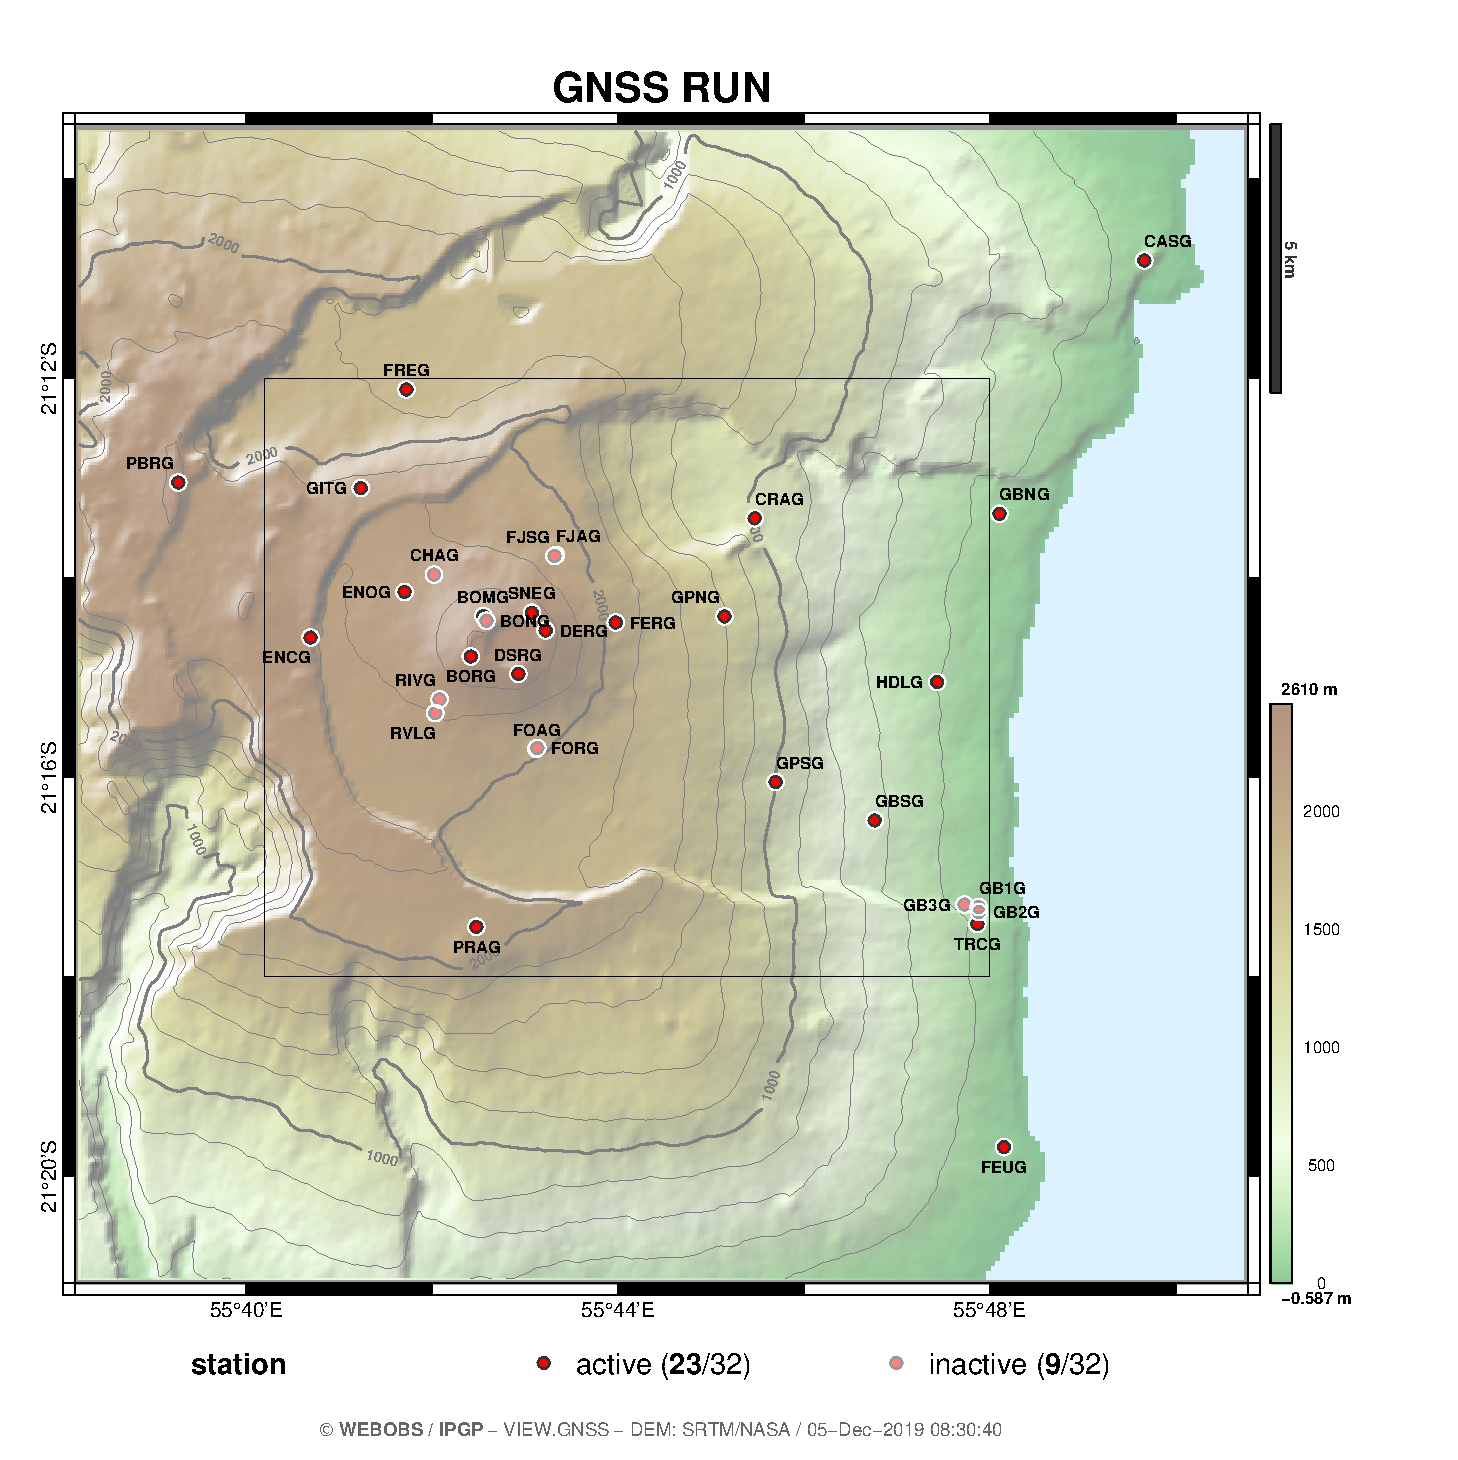
\includegraphics[width=\textwidth]{./VIEW.GNSS_map.eps}};
		
		% styles
		\tikzstyle{myLabel}=[draw=black, circle, fill=white, inner sep=0pt, minimum size=5pt]
		\tikzstyle{myLine}=[draw=blue,  double]	
		
		\node[myLabel] (CASG) at (3.5,4) {} ;
		\node[myLabel] (GBNG) at (2.3,1.85) {} ;
		\node[myLabel] (FREG) at (-2.75,2.9) {} ;
		\node[myLabel] (PBRG) at (-4.7,2.1) {} ;
		\node[myLabel] (CRAG) at (0.2,1.8) {} ;
		\node[myLabel] (GITG) at (-3.15,2.05) {} ;
		\node[myLabel] (ENCG) at (-3.55,.8) {} ;
		\node[myLabel] (ENOG) at (-2.75,1.15) {} ;
		\node[myLabel] (BOMG) at (-2.1,.99) {} ;
		\node[myLabel] (SNEG) at (-1.7,1) {} ;
		\node[myLabel] (DERG) at (-1.55,.85) {} ;
		\node[myLabel] (FERG) at (-.95,.9) {} ;
		\node[myLabel] (GPNG) at (-.05,.95) {} ;
		\node[myLabel] (HDLG) at (1.75,.4) {} ;
		\node[myLabel] (BORG) at (-2.2,.64) {} ;
		\node[myLabel] (DSRG) at (-1.8,.46) {} ;
		\node[myLabel] (GPSG) at (.4,-.45) {} ;
		\node[myLabel] (GBSG) at (1.25,-.75) {} ;
		\node[myLabel] (PRAG) at (-2.15,-1.66) {} ;
		\node[myLabel] (GB1G) at (2.15,-1.5) {} ;
		\node[myLabel] (TRCG) at (2.1,-1.65) {} ;
		\node[myLabel] (FOAG) at (-1.64,-.15) {} ;
		\node[myLabel] (RVLG) at (-2.48,0.13) {} ;
		\node[myLabel] (FJAG) at (-1.45,1.5) {};
		\node[myLabel] (FEUG) at (2.35,-3.55) {};
		
		\loaddata{../results/edges_GNSS_StudentGL.dat}
		\foreach \start/\dest  in \loadeddata{
			\path[myLine] (\start) -- (\dest);
		}
		\node[star,star point ratio=2,minimum size=7pt,
		inner sep=0pt,draw=black,solid,fill=red] at (-2.06,.75) {};
		
	\end{tikzpicture}

	\begin{tikzpicture}
		\draw (0,0) node[inner sep=0] {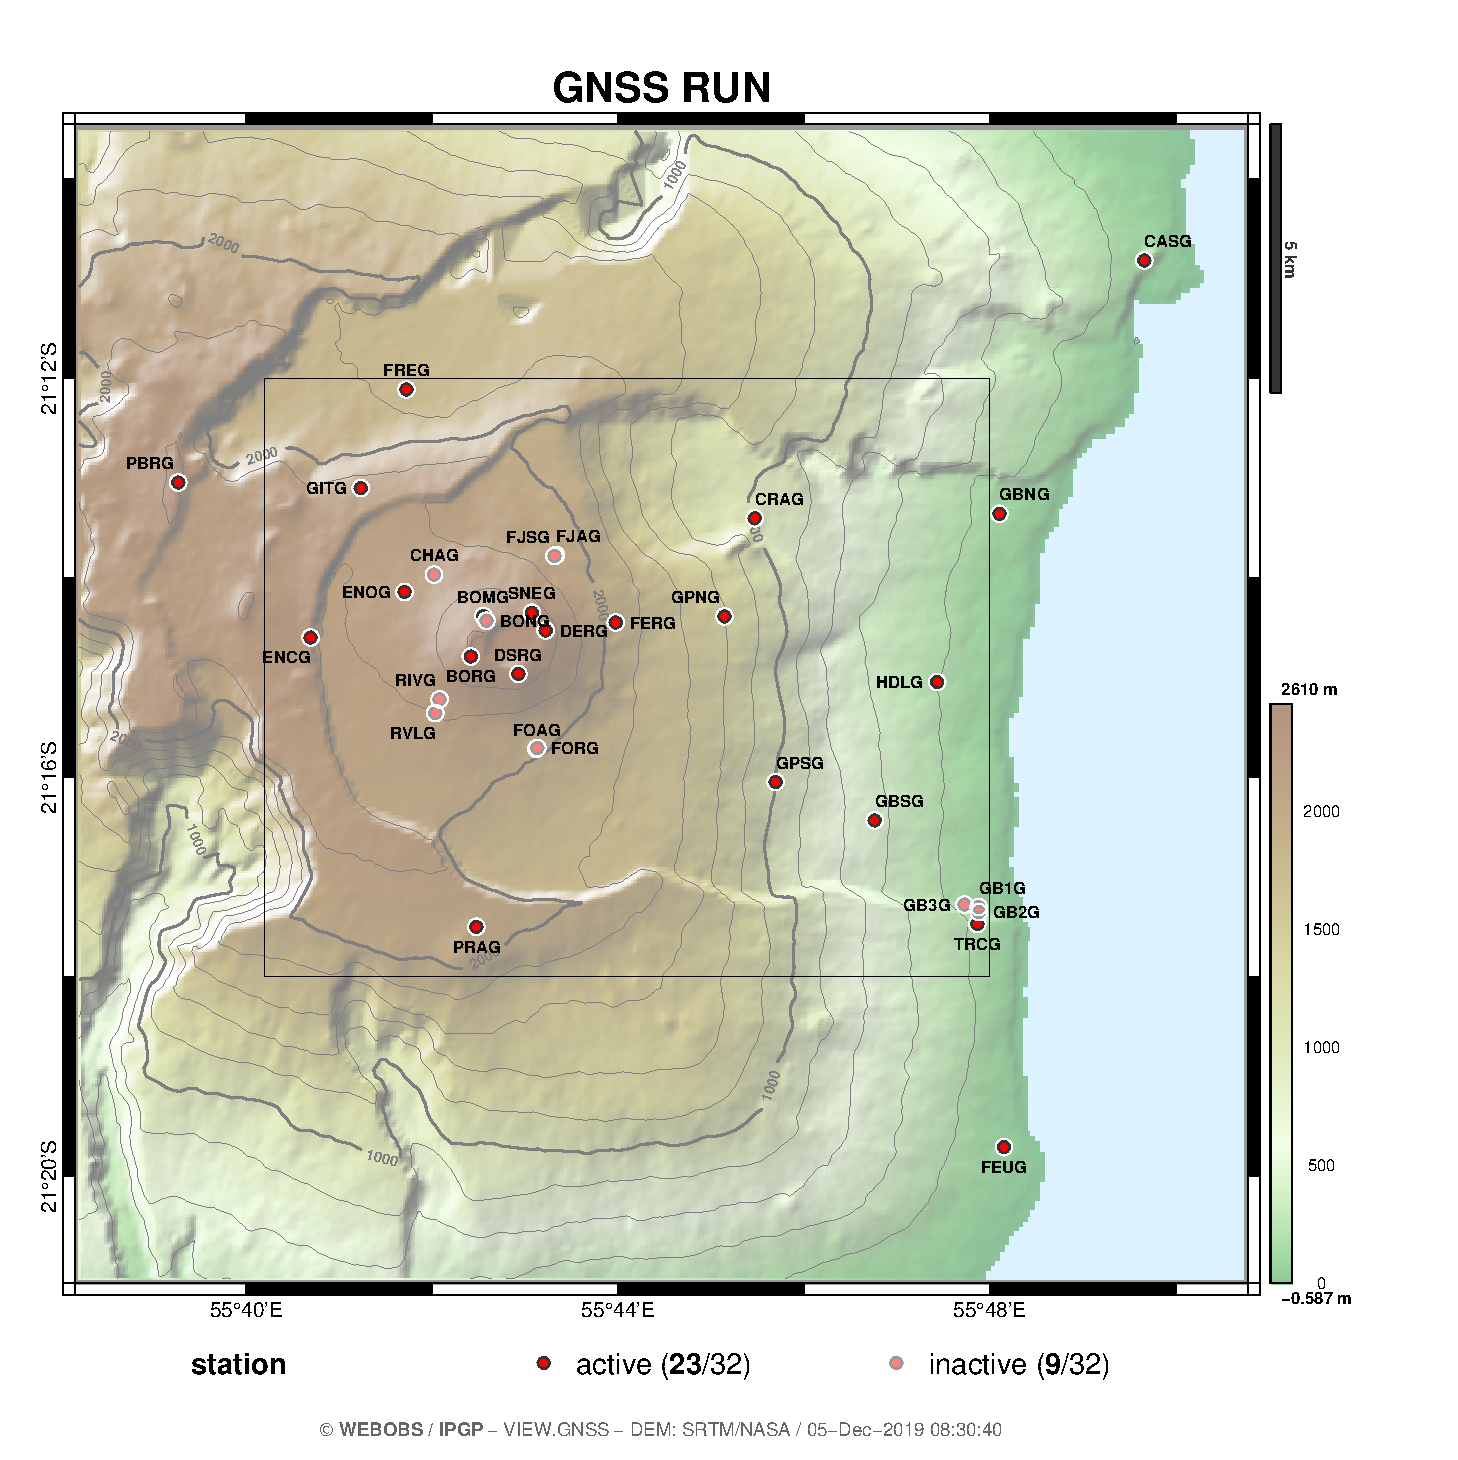
\includegraphics[width=\textwidth]{./VIEW.GNSS_map.eps}};
		
		% styles
		\tikzstyle{myLabel}=[draw=black, circle, fill=white, inner sep=0pt, minimum size=5pt]
		\tikzstyle{myLine}=[draw=blue,  double]	
		
		\node[myLabel] (CASG) at (3.5,4) {} ;
		\node[myLabel] (GBNG) at (2.3,1.85) {} ;
		\node[myLabel] (FREG) at (-2.75,2.9) {} ;
		\node[myLabel] (PBRG) at (-4.7,2.1) {} ;
		\node[myLabel] (CRAG) at (0.2,1.8) {} ;
		\node[myLabel] (GITG) at (-3.15,2.05) {} ;
		\node[myLabel] (ENCG) at (-3.55,.8) {} ;
		\node[myLabel] (ENOG) at (-2.75,1.15) {} ;
		\node[myLabel] (BOMG) at (-2.1,.99) {} ;
		\node[myLabel] (SNEG) at (-1.7,1) {} ;
		\node[myLabel] (DERG) at (-1.55,.85) {} ;
		\node[myLabel] (FERG) at (-.95,.9) {} ;
		\node[myLabel] (GPNG) at (-.05,.95) {} ;
		\node[myLabel] (HDLG) at (1.75,.4) {} ;
		\node[myLabel] (BORG) at (-2.2,.64) {} ;
		\node[myLabel] (DSRG) at (-1.8,.46) {} ;
		\node[myLabel] (GPSG) at (.4,-.45) {} ;
		\node[myLabel] (GBSG) at (1.25,-.75) {} ;
		\node[myLabel] (PRAG) at (-2.15,-1.66) {} ;
		\node[myLabel] (GB1G) at (2.15,-1.5) {} ;
		\node[myLabel] (TRCG) at (2.1,-1.65) {} ;
		\node[myLabel] (FOAG) at (-1.64,-.15) {} ;
		\node[myLabel] (RVLG) at (-2.48,0.13) {} ;
		\node[myLabel] (FJAG) at (-1.45,1.5) {};
		\node[myLabel] (FEUG) at (2.35,-3.55) {};
		
		\loaddata{../results/edges_GNSS_GGM.dat}
		\foreach \start/\dest  in \loadeddata{
			\path[myLine] (\start) -- (\dest);
		}
		\node[star,star point ratio=2,minimum size=7pt,
		inner sep=0pt,draw=black,solid,fill=red] at (-2.06,.75) {};
		
	\end{tikzpicture}

\begin{tikzpicture}
	\draw (0,0) node[inner sep=0] {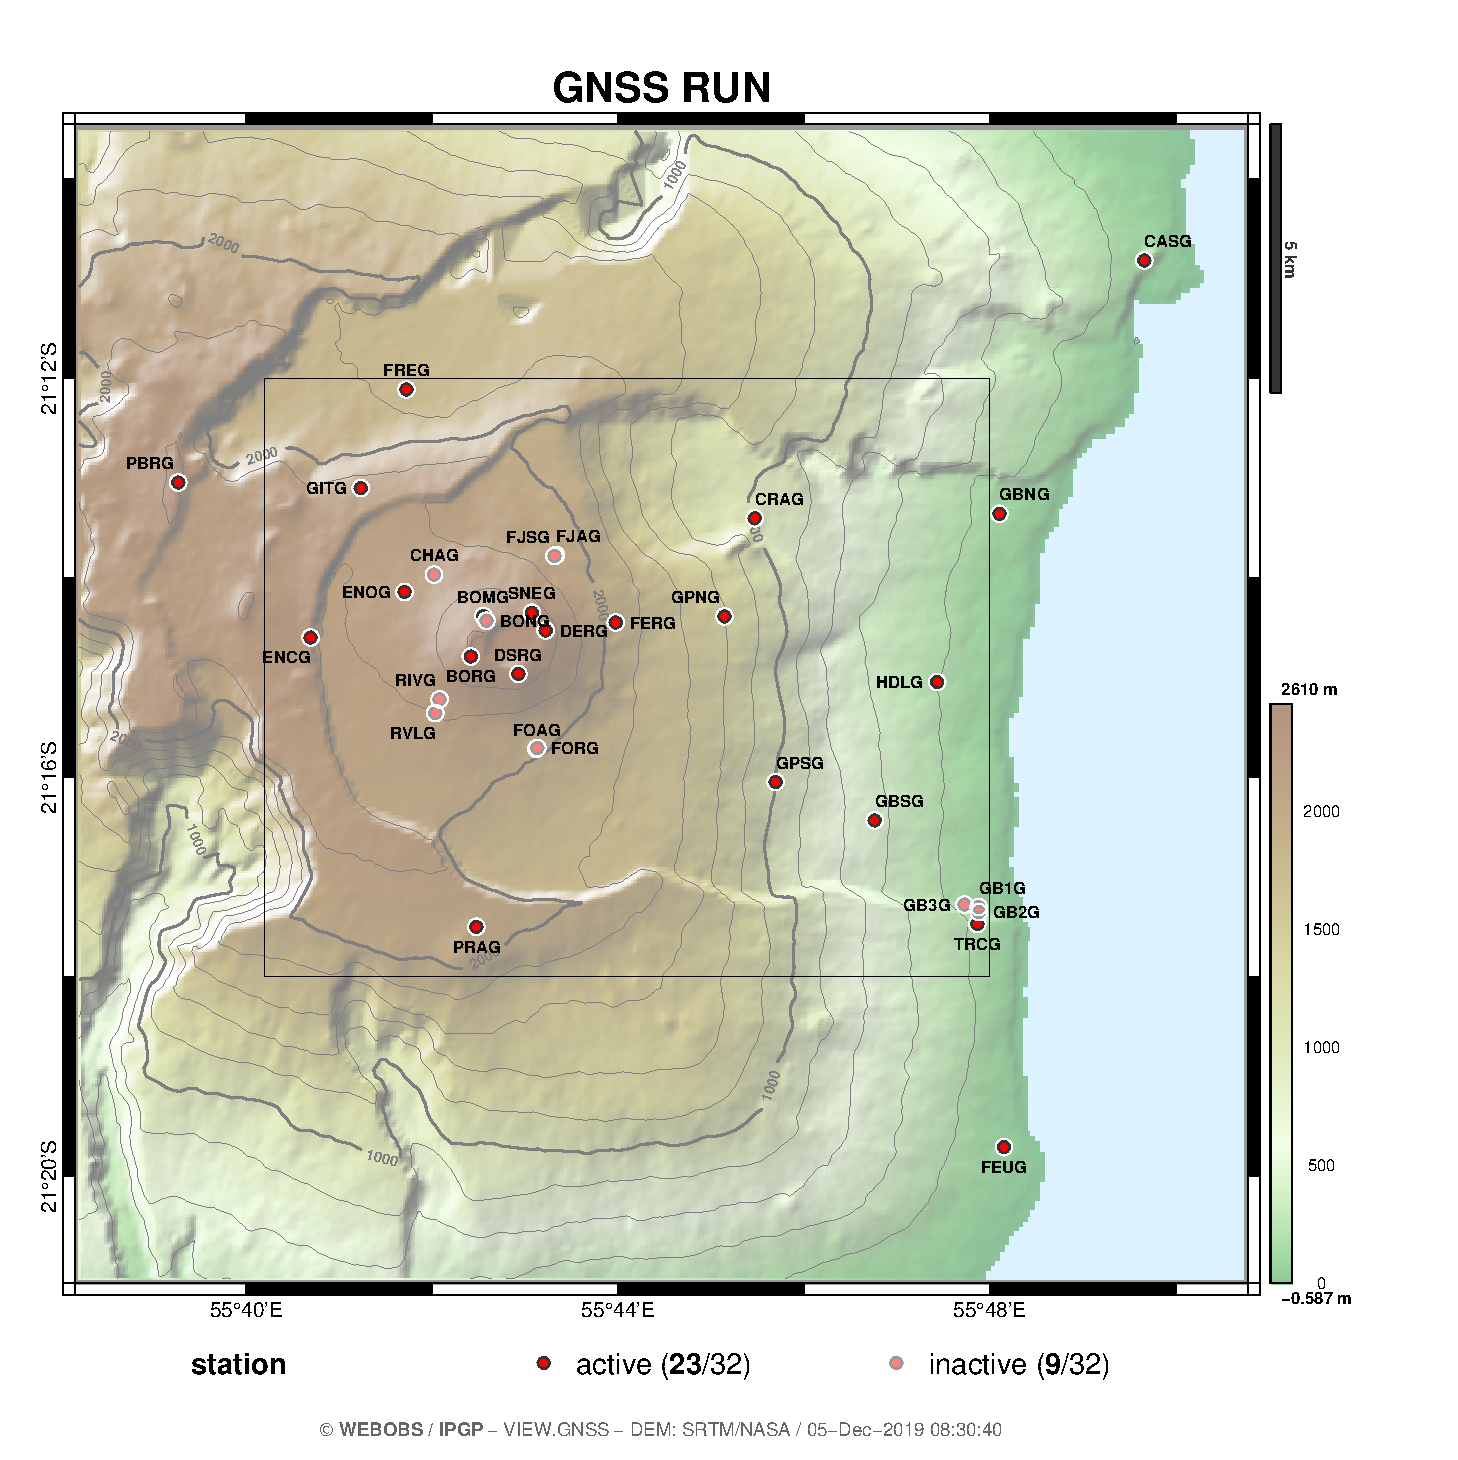
\includegraphics[width=\textwidth]{./VIEW.GNSS_map.eps}};
	
	% styles
	\tikzstyle{myLabel}=[draw=black, circle, fill=white, inner sep=0pt, minimum size=5pt]
	\tikzstyle{myLine}=[draw=blue,  double]	
	
	\node[myLabel] (CASG) at (3.5,4) {} ;
	\node[myLabel] (GBNG) at (2.3,1.85) {} ;
	\node[myLabel] (FREG) at (-2.75,2.9) {} ;
	\node[myLabel] (PBRG) at (-4.7,2.1) {} ;
	\node[myLabel] (CRAG) at (0.2,1.8) {} ;
	\node[myLabel] (GITG) at (-3.15,2.05) {} ;
	\node[myLabel] (ENCG) at (-3.55,.8) {} ;
	\node[myLabel] (ENOG) at (-2.75,1.15) {} ;
	\node[myLabel] (BOMG) at (-2.1,.99) {} ;
	\node[myLabel] (SNEG) at (-1.7,1) {} ;
	\node[myLabel] (DERG) at (-1.55,.85) {} ;
	\node[myLabel] (FERG) at (-.95,.9) {} ;
	\node[myLabel] (GPNG) at (-.05,.95) {} ;
	\node[myLabel] (HDLG) at (1.75,.4) {} ;
	\node[myLabel] (BORG) at (-2.2,.64) {} ;
	\node[myLabel] (DSRG) at (-1.8,.46) {} ;
	\node[myLabel] (GPSG) at (.4,-.45) {} ;
	\node[myLabel] (GBSG) at (1.25,-.75) {} ;
	\node[myLabel] (PRAG) at (-2.15,-1.66) {} ;
	\node[myLabel] (GB1G) at (2.15,-1.5) {} ;
	\node[myLabel] (TRCG) at (2.1,-1.65) {} ;
	\node[myLabel] (FOAG) at (-1.64,-.15) {} ;
	\node[myLabel] (RVLG) at (-2.48,0.13) {} ;
	\node[myLabel] (FJAG) at (-1.45,1.5) {};
	\node[myLabel] (FEUG) at (2.35,-3.55) {};
	
	\loaddata{../results/edges_GNSS_EGM.dat}
	\foreach \start/\dest  in \loadeddata{
		\path[myLine] (\start) -- (\dest);
	}
	\node[star,star point ratio=2,minimum size=7pt,
	inner sep=0pt,draw=black,solid,fill=red] at (-2.06,.75) {};
	
\end{tikzpicture}

\begin{tikzpicture}
	\draw (0,0) node[inner sep=0] {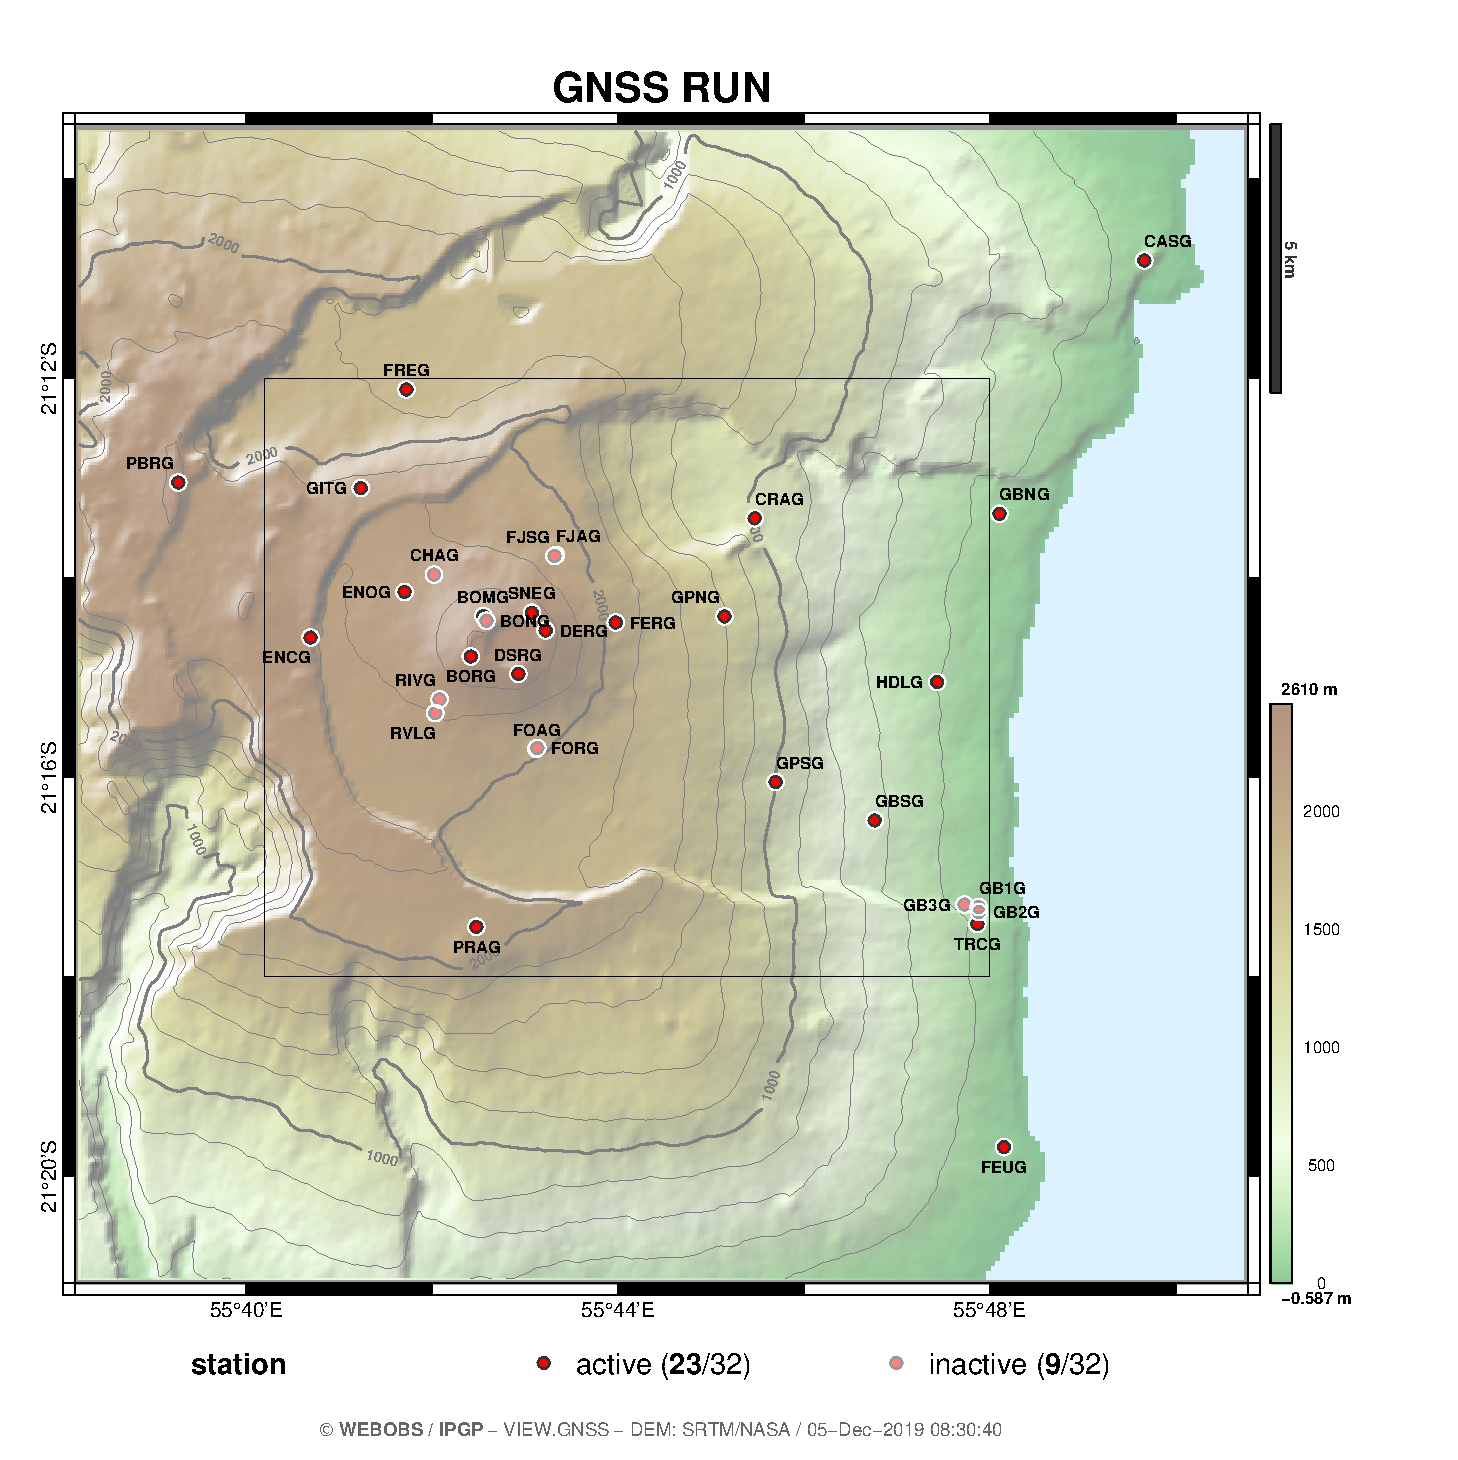
\includegraphics[width=\textwidth]{./VIEW.GNSS_map.eps}};
	
	% styles
	\tikzstyle{myLabel}=[draw=black, circle, fill=white, inner sep=0pt, minimum size=5pt]
	\tikzstyle{myLine}=[draw=blue,  double]	
	
	\node[myLabel] (CASG) at (3.5,4) {} ;
	\node[myLabel] (GBNG) at (2.3,1.85) {} ;
	\node[myLabel] (FREG) at (-2.75,2.9) {} ;
	\node[myLabel] (PBRG) at (-4.7,2.1) {} ;
	\node[myLabel] (CRAG) at (0.2,1.8) {} ;
	\node[myLabel] (GITG) at (-3.15,2.05) {} ;
	\node[myLabel] (ENCG) at (-3.55,.8) {} ;
	\node[myLabel] (ENOG) at (-2.75,1.15) {} ;
	\node[myLabel] (BOMG) at (-2.1,.99) {} ;
	\node[myLabel] (SNEG) at (-1.7,1) {} ;
	\node[myLabel] (DERG) at (-1.55,.85) {} ;
	\node[myLabel] (FERG) at (-.95,.9) {} ;
	\node[myLabel] (GPNG) at (-.05,.95) {} ;
	\node[myLabel] (HDLG) at (1.75,.4) {} ;
	\node[myLabel] (BORG) at (-2.2,.64) {} ;
	\node[myLabel] (DSRG) at (-1.8,.46) {} ;
	\node[myLabel] (GPSG) at (.4,-.45) {} ;
	\node[myLabel] (GBSG) at (1.25,-.75) {} ;
	\node[myLabel] (PRAG) at (-2.15,-1.66) {} ;
	\node[myLabel] (GB1G) at (2.15,-1.5) {} ;
	\node[myLabel] (TRCG) at (2.1,-1.65) {} ;
	\node[myLabel] (FOAG) at (-1.64,-.15) {} ;
	\node[myLabel] (RVLG) at (-2.48,0.13) {} ;
	\node[myLabel] (FJAG) at (-1.45,1.5) {};
	\node[myLabel] (FEUG) at (2.35,-3.55) {};
	
	\loaddata{../results/edges_GNSS_GGFM.dat}
	\foreach \start/\dest  in \loadeddata{
		\path[myLine] (\start) -- (\dest);
	}
	\node[star,star point ratio=2,minimum size=7pt,
	inner sep=0pt,draw=black,solid,fill=red] at (-2.06,.75) {};
	
\end{tikzpicture}

\begin{tikzpicture}
	\draw (0,0) node[inner sep=0] {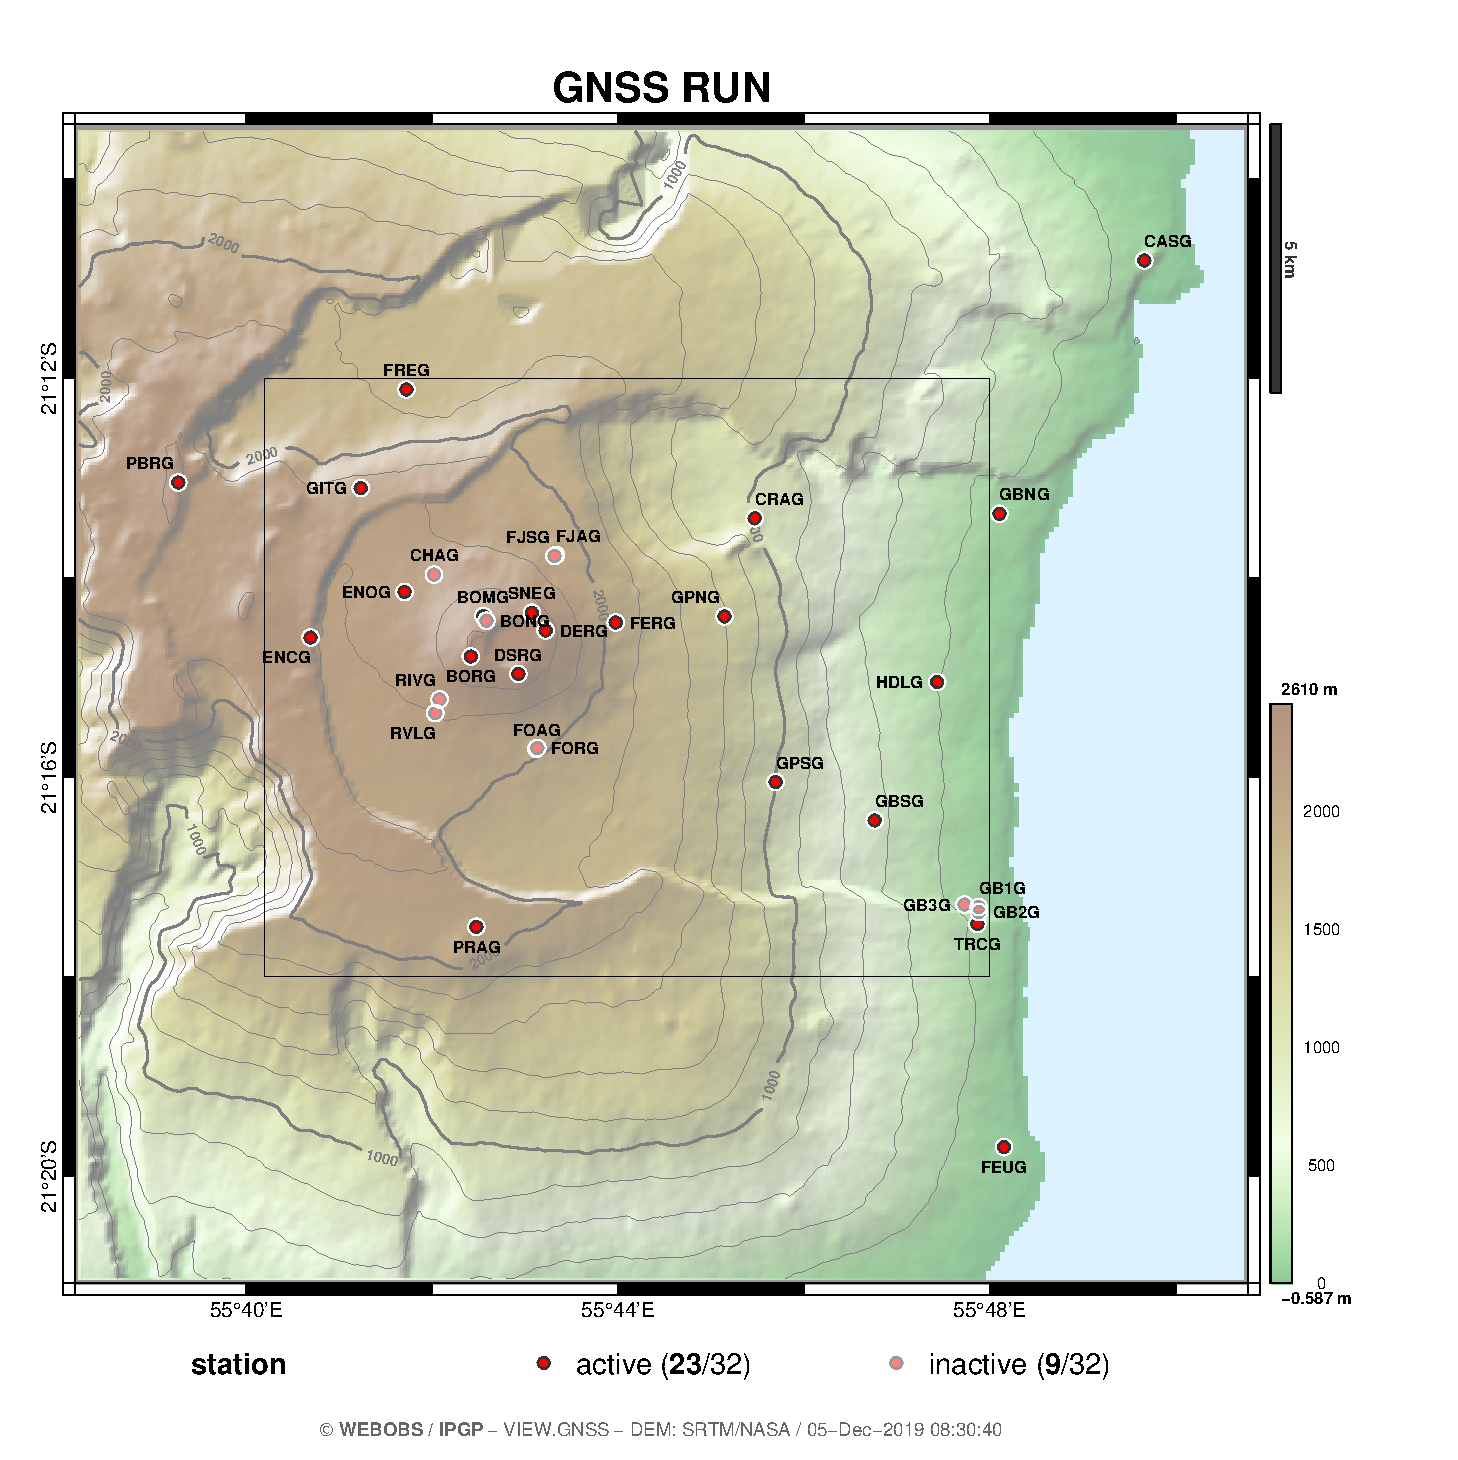
\includegraphics[width=\textwidth]{./VIEW.GNSS_map.eps}};
	
	% styles
	\tikzstyle{myLabel}=[draw=black, circle, fill=white, inner sep=0pt, minimum size=5pt]
	\tikzstyle{myLine}=[draw=blue,  double]	
	
	\node[myLabel] (CASG) at (3.5,4) {} ;
	\node[myLabel] (GBNG) at (2.3,1.85) {} ;
	\node[myLabel] (FREG) at (-2.75,2.9) {} ;
	\node[myLabel] (PBRG) at (-4.7,2.1) {} ;
	\node[myLabel] (CRAG) at (0.2,1.8) {} ;
	\node[myLabel] (GITG) at (-3.15,2.05) {} ;
	\node[myLabel] (ENCG) at (-3.55,.8) {} ;
	\node[myLabel] (ENOG) at (-2.75,1.15) {} ;
	\node[myLabel] (BOMG) at (-2.1,.99) {} ;
	\node[myLabel] (SNEG) at (-1.7,1) {} ;
	\node[myLabel] (DERG) at (-1.55,.85) {} ;
	\node[myLabel] (FERG) at (-.95,.9) {} ;
	\node[myLabel] (GPNG) at (-.05,.95) {} ;
	\node[myLabel] (HDLG) at (1.75,.4) {} ;
	\node[myLabel] (BORG) at (-2.2,.64) {} ;
	\node[myLabel] (DSRG) at (-1.8,.46) {} ;
	\node[myLabel] (GPSG) at (.4,-.45) {} ;
	\node[myLabel] (GBSG) at (1.25,-.75) {} ;
	\node[myLabel] (PRAG) at (-2.15,-1.66) {} ;
	\node[myLabel] (GB1G) at (2.15,-1.5) {} ;
	\node[myLabel] (TRCG) at (2.1,-1.65) {} ;
	\node[myLabel] (FOAG) at (-1.64,-.15) {} ;
	\node[myLabel] (RVLG) at (-2.48,0.13) {} ;
	\node[myLabel] (FJAG) at (-1.45,1.5) {};
	\node[myLabel] (FEUG) at (2.35,-3.55) {};
	
	\loaddata{../results/edges_GNSS_EGFM.dat}
	\foreach \start/\dest  in \loadeddata{
		\path[myLine] (\start) -- (\dest);
	}
	\node[star,star point ratio=2,minimum size=7pt,
	inner sep=0pt,draw=black,solid,fill=red] at (-2.06,.75) {};
	
\end{tikzpicture}

	

\end{document}